\begin{frame}{What is a Microcontroller?}
    \par Microcontroller is a computer system in a single chip.
    \par Just like a \acs{pc}, it consists of:
    \begin{itemize}
        \item \acs{cpu} --- less powerful than a full blown desktop processor
        \item Persistent and non-persistent memory (\acs{hdd}, \acs{ram}) --- typically a few \SI{100}{\kibi\byte} of \acs{ram} instead of > \SI{1}{\gibi\byte} like a typical computer
        \item System clock --- not as fast as desktop processors, but many \acsp{uc} can also be clocked externally
        \item Peripherals --- provide interfaces found in the field of embedded systems (\acs{gpio}, \acs{i2c}, \acs{spi}, \acs{uart}, \acs{can}, \ldots) rather than interfaces found in desktop computers (\acs{pci}, \acs{pcie}, Thunderbolt \texttrademark, \acs{sata}, \ldots)
    \end{itemize}
\end{frame}

\begin{frame}{What is a Microcontroller?}
    \begin{figure}
        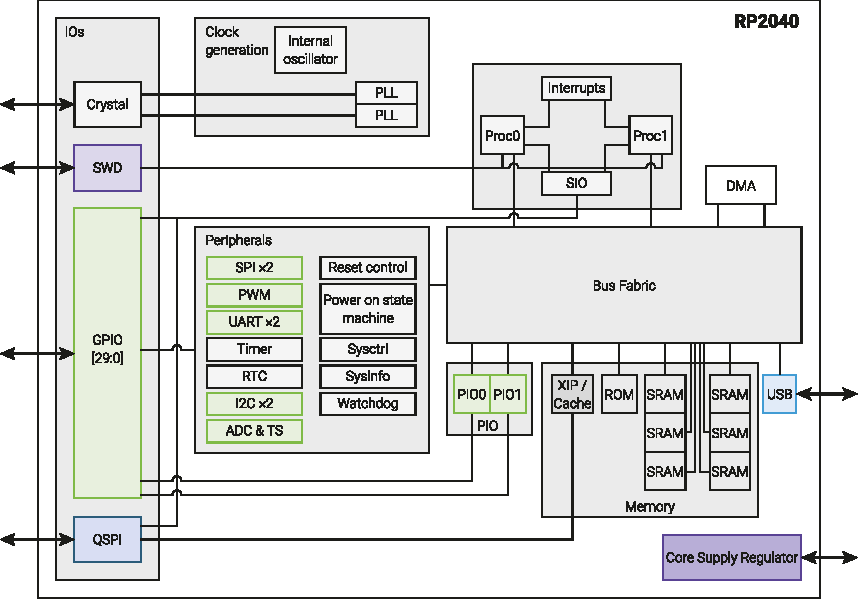
\includegraphics[width=0.9\textwidth]{microcontroller/arduino/rp2040/block-diagram.pdf}
        \caption{System overview of the RP2040 Chip}
    \end{figure}
\end{frame}

\begin{frame}{What is a Microcontroller?}
    \begin{figure}
        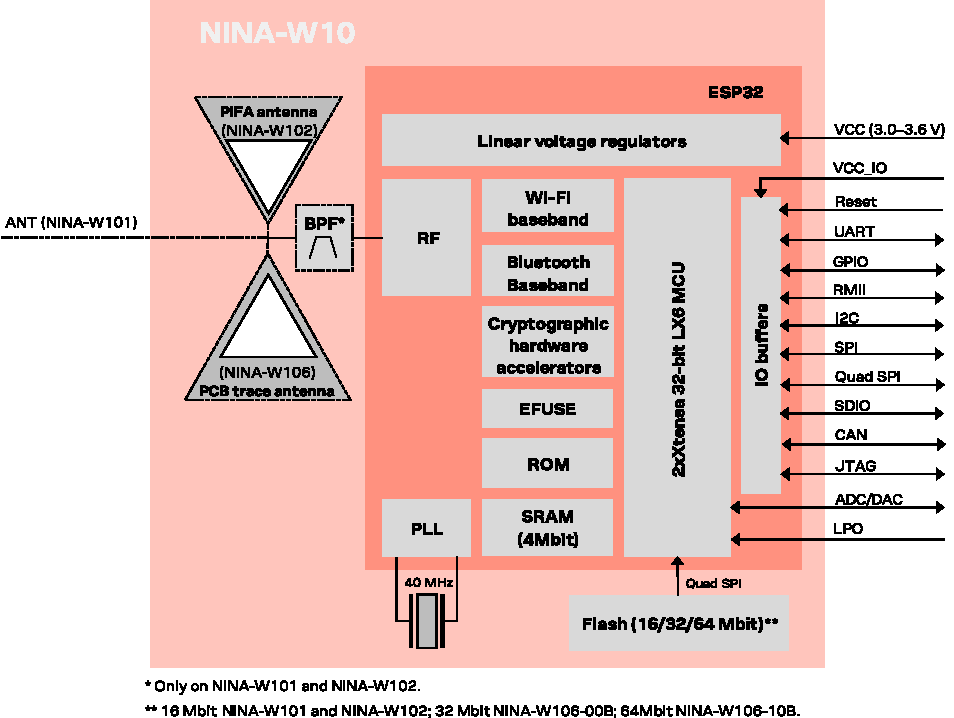
\includegraphics[width=0.9\textwidth]{microcontroller/nina-w10-block-diagram.pdf}
        \caption{Nina W10 Block Diagram}
    \end{figure}
\end{frame}

\begin{frame}{What is a Microcontroller?}
    \begin{figure}
        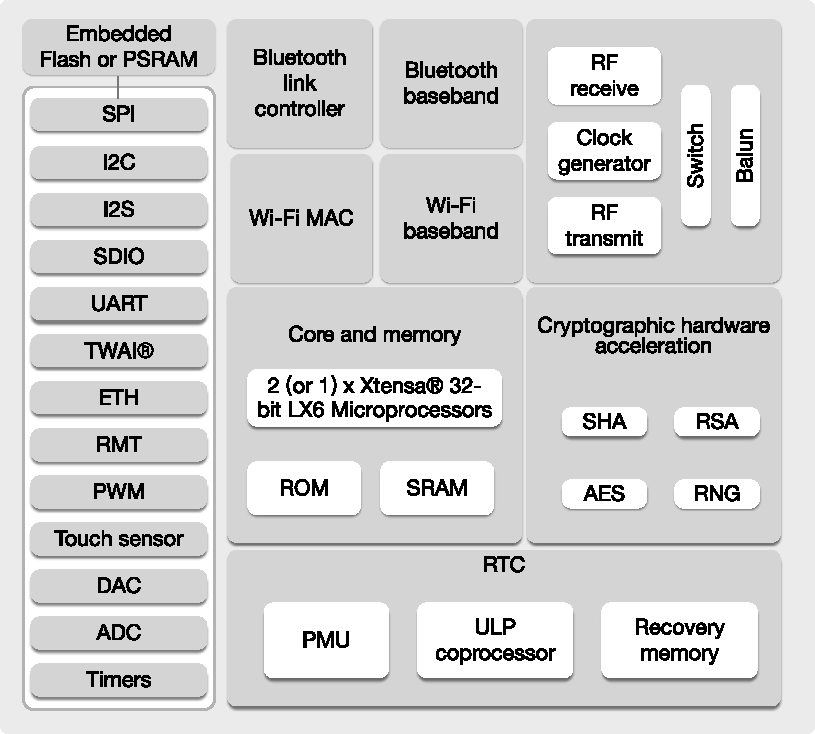
\includegraphics[width=0.7\textwidth]{microcontroller/esp32-functional-block-diagram.pdf}
        \caption{ESP32 Functional Block Diagram}
    \end{figure}
\end{frame}

\begin{frame}{What is a Microcontroller?}
    \begin{itemize}
        \item A \acf{mcu} is a compact integrated circuit designed to govern specific operations in an embedded system.
        \item Unlike a general-purpose computer, a microcontroller performs a focused set of tasks, often with \textit{real-time} constraints.
        \item Core Components:
        \begin{itemize}
            \item \textbf{Central Processing Unit (CPU)}: Executes program instructions stored in memory.
            \item \textbf{Memory}:
                \begin{itemize}
                    \item \textit{Program Memory (Flash)}: Stores the program code.
                    \item \textit{Data Memory (\acs{ram})}: Stores temporary data.
                \end{itemize}
            \item \textbf{\acf{io} Peripherals}: Interfaces with other parts of the system, like sensors, displays, etc.
            \item \textbf{Other peripherals}: Timers, communication ports, etc.
        \end{itemize}
        \item Microcontrollers are often described by their memory size, and the nature and number of \acs{io} ports and peripherals.
    \end{itemize}
\end{frame}

\begin{frame}{Comparing \glsentrytext{mcu}, \glsentrytext{mpu}, and \glsentrytext{dsp}}
    \begin{table}
        \resizebox{\linewidth}{!}{
            \begin{tblr}{width=1.5\linewidth, colspec={X[2]X[3]X[3]X[3]}, hlines, row{1}={font=\bf}}
                Aspect               & \acs{mcu}                                & \acs{mpu}                                 & \acs{dsp} \\
                Purpose              & Specific tasks                           & General computing                         & Signal processing \\
                \acs{cpu}            & Integrated                               & Separate                                  & Specialized \\
                Memory               & On-chip                                  & External                                  & Often on-chip \\
                \acs{io} Ports       & Integrated                               & External                                  & Integrated/External \\
                Cost                 & Lower                                    & Higher                                    & Varies \\
                Complexity           & Lower                                    & Higher                                    & Moderate \\
                Performance          & Moderate                                 & High                                      & High (in signal processing) \\
                Application \newline Examples & Embedded systems, \newline automation    & \acs{pc}, Servers, \newline workstations  & Audio processing, \newline image processing \\
            \end{tblr}
        }
    \end{table}
\end{frame}